\documentclass[12pt,twoside]{report}

\usepackage{color}
\usepackage{graphicx}                   
\DeclareGraphicsExtensions{.eps,.ps}               

\topmargin -0.3in
\oddsidemargin 0.5in
\evensidemargin 0.5in
\textheight 8.5in
\textwidth 6.0in
%
% ====================================================================
%     The following commands tend to keep LaTex happier in the 
%     placement of figures, tables, etc
% ====================================================================
%
\renewcommand{\textfraction}{0.0}
\renewcommand{\floatpagefraction}{0.0}
\renewcommand{\topfraction}{1.0}
\renewcommand{\bottomfraction}{1.0}
\setcounter{topnumber}{9}
\setcounter{bottomnumber}{9}
\setcounter{totalnumber}{9}
% 
% ====================================================================
%     Some of the things we need for the title page
% ====================================================================
%
\author{\\
	\\
	\\
	by \\
	\\
      	Kiyotaka Akabori \\
	\\
	\\
	\\
	\\
	\\
        Submitted in partial fulfillment of the \\
        requirements for the degree of \\
        Doctor of Philosophy \\
        at \\
        Carnegie Mellon University \\
        Department of Physics \\
        Pittsburgh, Pennsylvania \\
	\\
        \\
	Advised by Professor John F. Nagle
	\\
	\\
}

\title{\bf{
Measurement of the Most Important Physics Quantity Ever Discovered 
}}

\date{\today}

%
% ====================================================================
%     Input your definition in file definitions.tex here. 
%     A simple example of the content of such a file is given below.
% ====================================================================
%
%\input{definitions}
%
%%%%%%%%%%%%%% Example for content of file definitions.tex %%%%%%%%%%%
\def\ra    {\rightarrow}
\def\ul    {\underline} 
\def\mevcc {\ifmmode {\mathrm MeV}/c^2 \else MeV$/c^2$\fi}
\def\BsJpsiPhi {\ensuremath{\Bs \ra J/\psi\,\phi}}
%%%%%%%%%%%%%%%%%%%%%%%%%%%%%%%%%%%%%%%%%%%%%%%%%%%%%%%%%%%%%%%%%%%%%%
%
\begin{document} 

\thispagestyle{empty}

\maketitle

% ====================================================================
%     Generates one blank page before the 'Abstract'
% ====================================================================

\thispagestyle{empty} \cleardoublepage

%
\begin{abstract}

  This is the most important discovery made in the history of modern
  physics. We discuss the detailed measurement that solved the mystery
  of the universe.  This is the most important discovery made in the
  history of modern physics. We discuss the detailed measurement that
  solved the mystery of the universe.  This is the most important
  discovery made in the history of modern physics. We discuss the
  detailed measurement that solved the mystery of the universe.
  
\end{abstract}

%


\thispagestyle{empty} \cleardoublepage

\pagenumbering{roman}

%
\section*{Acknowledgments}

I would like to thank my advisors Profs. John F. Nagle and Stephanie
Tristram-Nagle for giving me an opportunity to work in the field of biophysics,
for guiding my research, and for supporting me as a research assistant. 

I especially thank Michael S. Jablin for a number of exciting discussions and 
projects we shared. Despite our differences, he always respected my opinions
and helped me shape my ideas.

I thank Profs. Angel E. Garc\'{i}a, Robert M. Suter, and Frank Heinrich
for serving on my Ph.D. committee.

Thanks to Dr. Kun Huang for providing us with many simulation results.

I thank Prof. Christian D. Santangelo for giving me a chance to work on 
a theoretical problem. 

Many thanks to my wife for the countless moments of joy and laughter,
supporting my Ph.D. study with great meals every day, and being a wonderful 
mother.
And to Shyn, I am so proud to be your father.

%


\tableofcontents 

\listoftables

\listoffigures

\clearpage 

\pagenumbering{arabic}

%
\chapter{Introduction}
\section{Lipid bilayer}
In biological system, cell membranes define the boundary of living organism
and surrounding environment. They regulate what can come and leave living
cells. Building blocks of cell membranes are lipid bilayers.
Lipid bilayers are self-assembled system of lipids, which are 
amphiphilic molecules, consisting of a hydrophilic headgroup
and hydrophobic chains (Fig.~\ref{fig:lipid}).

\begin{figure}
  \centering
  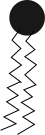
\includegraphics[width=0.05\textwidth]{figures/lipid}
  \caption{Schematic representation of a lipid molecule}
  \label{fig:lipid}
\end{figure}

In water lipids self-assemble into lipid bilayes to shield their hydrophobic 
cores, and 
display a wide variety of thermodynamic phases
as a function of temperature and hydration. Figure~\ref{fig:phase_diagram}
shows a phase diagram of dimyristoylphosphatidylcholines (DMPC).
PC lipids constitute a substantial fraction of cell membranes
and have been studied for many decades.
At full hydration, a lamellar phase coexists with excess water.
In the high temperature, fluid L$_\alpha$ phase, the hydrocarbon chains 
are conformationally disordered, and intra-membrane molecular correlations 
are liquid-like \cite{ref:Fahey78} (Fig.~\ref{fig:various_phases}).
Disordering and flexibility of fluid phase membranes allow them to 
interact with proteins in various ways, leading to the complex nature
of biological systems. 
This phase is usually considered biologically relevant, making it
the most widely studied phase for understanding various biological processes.

\begin{figure}[htbp]
  \centering
  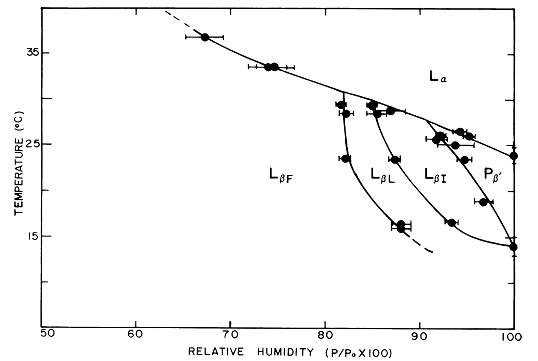
\includegraphics[width=0.9\textwidth]{figures/ripple/smith_phase_diagram}
  \caption{Experimental phase diagram of DMPC from Ref.~\cite{ref:Smith88}.
  \LbetaI, \LbetaL, and \LbetaF\ belong to the gel L$_{\beta'}$ phase. P$_{\beta'}$ is 
  the ripple phase and L$_\alpha$ is the fluid phase.}
  \label{fig:phase_diagram}
\end{figure}

\begin{figure}[htbp]
  \centering
  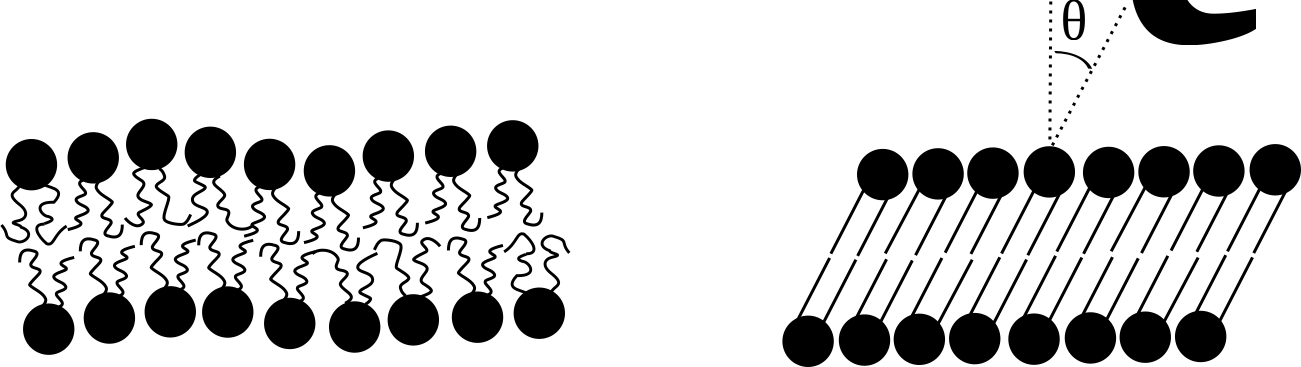
\includegraphics[width=0.9\textwidth]{figures/ripple/various_phases}
  \caption[]{Schematics of the structure of fluid L$_\alpha$ phase (left) and 
  gel L$_{\beta'}$ phase (right). Black solid circles are lipid headgroups 
  and solid lines are lipid chains. $\theta_t$ is the chain tilt angle.}
  \label{fig:various_phases}
\end{figure}

In the low temperature, gel L$_{\beta'}$
phase, hydrocarbon chains are stiff and titled with respect to the membrane
normal \cite{ref:Tardieu73}, and are organized in a either hexagonal 
or orthorhombic lattice. 
The L$_{\beta'}$ is further categorized into three phases according to the 
chain tilt direction \cite{ref:Smith88}. 
In the L$_{\beta\text{I}}$ phase, chains are titled toward the 
nearest neighbor as shown in Fig.~\ref{fig:gel_phase_packing}, and
in the \LbetaF\ phase, chains are titled toward the next-next nearest neighbor.
In the \LbetaL\ phase, chains are tilted toward an intermediate direction.

\begin{figure}[htbp]
  \centering
  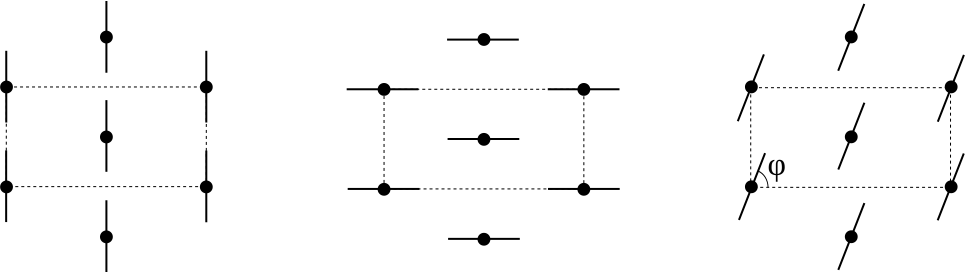
\includegraphics[width=0.9\textwidth]{figures/ripple/gel_phase_packing}
  \caption{Chain tilt direction in \LbetaI\ (left), \LbetaF\ (middle), and
  \LbetaL\ (right) phases. Black dots are orthorhombic lattice points.
  Unit cells are shown in dashed lines.
  Chains are drawn as solid lines. Chains are tilted toward the
  nearest neighbor in \LbetaI\ phase with $\phi=\pi/2$. 
  In \LbetaF\ phase, they are titled toward the next-next nearest neighbor
  ($\phi=0$). In \LbetaL\ phase, $\phi$ can be anywhere between 0 and $\pi/2$.}
  \label{fig:gel_phase_packing}
\end{figure}

Between the fluid and gel phases appears a height modulated phase where
bilayers are no longer flat (Fig.~\ref{fig:ripple_cartoon}). 
The low angle diffraction pattern of this phase conforms to the symmetry
of a two dimensional monoclinic lattice. This phase was termed P$_\beta'$ 
and is commonly
called the ripple phase. The P$_{\beta'}$--L$_{\beta'}$ transition is often
called the pre-transition.
The topography of the membrane ripples has been directly
visualized by freeze fracture electron microscopy experiments 
\cite{ref:Luna77,ref:Copeland80,ref:Ruppel83,ref:Zasadzinski87,ref:Zasadzinski88}.
The wavelength of the modulation is about 140 \AA\ for 
dimyristoylphosphatidylcholine (DMPC),
which has 14 carbons in the hydrocarbon chains \cite{ref:Wack89}.
There has been evidence that molecular conformation in the ripple phase is not 
unique. NMR signals in the ripple phase \cite{ref:Wittebort81} were consistent
with a superposition of signals observed in the fluid and gel phases.
Lateral diffusion measurements found two distinct populations,
with diffusion coefficients characteristic of fluid and gel phases
\cite{ref:Schneider83}. 

\begin{figure}[htbp]
  \centering
  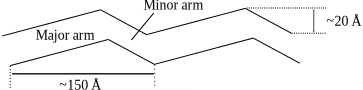
\includegraphics[width=0.7\textwidth]{figures/ripple/ripple_cartoon}
  \caption{Schematic of the P$_{\beta'}$ ripple phase. In this phase, 
  bilayers assume periodic height modulation with a sawtooth shape.
  The longer side of a sawtooth is called major arm and the shorter
  side is called minor arm. It is generally assumed that chains are
  in all trans conformation in the major arm, but the molecular packing
  in the minor arm is not known.}
  \label{fig:ripple_cartoon}
\end{figure}

There are various kinds of lipids. They can be 
categorized in terms of headgroup, chain saturation, and chain length.
The most studied headgroup is a phosphatidylcholine (PC),
consisting of phosphate and choline groups. Another class of headgroup is
anionic, phosphatidylserin (PS). In cells, electrostatic interaction 
greatly influence biological processes and naturally occurring anionic
lipids have been a focus of studies. More recently, membrane curvature
has attracted many physicists. Phosphatidylethanolamine (PE) is a small 
headgroup, and packing of PE lipids leads to spontaneous membrane curvature.
Many proteins have been found to sense/induce membrane curvature, 
making PE lipids especially attractive for those studies.
Lipid hydrocarbon chains can have one or more double bonds. Lipids
with no double bonds in the chains are called saturated lipids.
An example of such lipids is DMPC and DPPC. DPPC at room temperature
forms a L$_{\beta'}$ gel phase.
Lipids with one double bond
are called mono-unsaturated lipids. Examples of such lipids are DOPC.
Unsaturation lead to packing frustration and lower the melting 
temperature. DOPC at room temperature forms a L$_{\alpha}$ fluid phase.
In mammalian cells, unsaturated chains make up a large number.
For example, in plasma membranes,

\section{Tat}
we investigated the interaction of Tat peptide with lipid bilayers. 
This study is discussed in chapter 2.

\section{ripple}
we measured the electron density profile of the lipid
bilayers using a stack of oriented bilayers. Using wide angle x-ray scattering
technique, we also investigated the chain packing within a bilayer. 
The ripple phase is discussed in chapter 3. 
%
\chapter{Materials and Methods}
This chapter describes parts of experimental techniques that are common
in both Tat and ripple phase projects.
These common parts are also the key experimental components that make
experiments on oriented samples successful. Experimental and theoretical
methods that are specific to each project are described in each
respective chapter.

\section{X-ray optics}
High resolution setup should be described.

Low resolution setup should be described.

\section{Hydration Chamber}
Probably the most important of all.
The chamber is sealed very tightly. We used helium to replace air. Air 
scattering is strong. 
Mylar window, cast scatteing in wide angle region. Helium. Peltier used to 
condense water in and out of the sample.  

The sample was placed on a Peltier element that was connected to a controllable 
power supply and a multimeter was connected to read off the applied
current. 
In order to achieve a desired hydration of the sample,
small current was applied to the Peltier. 
The applied current caused the Peltier surface to either heat or cool
depending on the direction of the current. The sample became less hydrated
with the heated Peltier surface while it became more hydrated with the
cooled Peltier surface.
The temperature gradient caused by the Peltier was negligible 
(less than 0.1 \textcelsius). The hydration level of the sample
was quantified by the average inter-bilayer distance, $D$-spacing,
which was measured by indexing observed peaks in X-ray scattering.

\section{Sample Preparation}
\subsection{Stock Solutions}
Synthesized lipids were purchased from Avanti Polar Lipids (Alabaster, AL) and 
used without further purification. Membrane mimics for Tat experiments 
were prepared by first 
dissolving lyophilized lipids in chloroform and then mixing these stock 
solutions to create the lipid compositions
DOPC, DOPC/DOPE (3:1), DOPC/DOPE (1:1), DOPC/DOPS (3:1) and nuclear membrane
mimic (POPC/POPE/POPS/SoyPI/Cholesterol, 69:15:2:4:11) (based on Ref. [37]). 
Peptide
(Y47GRKKRRQRRR57) was purchased in two separate lots from the Peptide Synthesis 
Facility
(University of Pittsburgh, Pittsburgh, PA); mass spectroscopy revealed greater
than 95\% 
purity. This Tat
peptide corresponds to residues (47-57) of the 86 residues in the Tat 
protein [6]. Tat was
dissolved in HPLC trifluoroethanol (TFE) and then mixed with lipid stock 
solutions in
chloroform to form mole fractions between 0.0044 and 0.108. Weight of Tat in 
these mole
fractions was corrected for protein content (the remainder being 8 
trifluoroacetate counter-ions
from the peptide synthesis). Solvents were removed by evaporation in the fume 
hood followed
by 2 hours in a vacuum chamber at room temperature.

\subsection{Thin Film Samples}

For Tat experiments, four mg dried lipid/peptide mixture was re-dissolved in HPLC chloroform/TFE 
(2:1 v:v)
for most of the lipid compositions. 
DOPC/DOPS (3:1) mixtures required
chloroform/HFP (1:1 v:v) in order to solubilize the negatively charged DOPS. 
200 $\mu$l of 4 mg
mixtures in solvents were plated onto silicon wafers (15x30x1 mm) via the rock 
and roll method
[38] to produce stacks of $\approx$1800 well-aligned bilayers; 
solvents were removed by 
evaporation in
the fume hood, followed by two hours under vacuum. Samples were prehydrated 
through the
vapor in polypropylene hydration chambers at 37 \degC for two to six hours 
directly before hydrating in the
thick-walled X-ray hydration chamber [39] for 0.5 to 1 hour. 

For ripple phase experiments, four mg DMPC powder was dissolved in 
140 $\mu$l chloroform/methanol (2:1 v:v) mixture. The solution was
plated onto silicon wafers similarly to Tat mixtures. 
The sample was annealed at 60 \textcelsius\ for approximately
6-10 hours just before the X-ray experiment. 
Then, the sample was trimmed to 1 mm for high
resolution and 5 mm for low resolution study. The temperature
was set to 18 \textcelsius. 

\section{CCD detector}
Data reduction and correction for charged coupled device (CCD) detector
are discribed in detail in \cite{ref:Burner}.

%
\chapter{Structural Perturbation on Lipid Bilayers Due to Tat Peptide}
As discussed in chapter 2, the two main techniques employed in this thesis 
were molecular dynamics (MD) simulation and low angle X-ray scattering (LAXS).
First, we discuss the results and analysis of diffuse X-ray scattering. The
general protocol was the following; LAXS data were fitted to a model X-ray
scattering pattern from a stack of flucutating membranes via NFIT program,
the analysis of which yielded the bending modulus, $K_C$, and the bulk
modulus, $B$. Dividing the experimenal data by the model, then, gave the 
absolute X-ray form factor, $|F(q_z)$, which is the Fourier transform
of bilayer electron density profile along the bilayer normal direction, $z$. 
We fitted $|F(q_z)|$ to a model density profile using the scattering density
profile (SDP) program. The SDP program allows us to model a bilayer density
according to volumentric spacing constraint. The advantage of this program is
that we can see fine details of bilayer structure such as an individual
head group, terminal methly, and so on. The model requires many parameters
that are not so well determined. We then constrain many parameters from
the past experimental data and MD simulations. This is discussed in 
section ?.

The second main method is MD simulation. From simulation trajectory, we 
calculated the so called simulated X-ray form factor using the SIMtoEXP
program (ref). The best matching simulation result was chosen as the best
prediciton of the bilayer structure. We, then, calculated many structural
details from the trajectory that were not accessible experimentally.   

Section X discusses the implication of the results obtained in the proceeding 
sections. While this study does not probe dynamics of Tat translocation,
it supports Tat's ability to interact with neutral membranes. This finding
is compared with recent studies on a single arginine molecule.

\section{Introduction}
The name cell-penetrating peptide (CPP) connotes a peptide that 
easily penetrates cell membranes (for Reviews see [1-3]). 

This thesis focuses on 
the transactivator of translation, Tat, from the HIV-1 virus, which plays a 
role in AIDS progression. Earlier work showed that the HIV-Tat 
protein (86 amino acids) was efficiently taken up by cells, and concentrations 
as low as 1 nM were sufficient to transactivate a reporter gene expressed from 
the HIV-1 promoter [4, 5]. It has been reported that Tat protein uptake does not 
require ATP [6]. Studies using inhibitors of different types of endocytosis, 
including clathrin and caveolae-mediated, or receptor-independent 
macropinocytosis reached the same conclusion that ATP mediated endocytosis is 
not involved in Tat protein permeation [7-10]. However, this issue is 
controversial, as other studies found evidence for endocytosis in Tat protein 
import [11-19]. Still other studies have concluded that an ATP requirement for 
Tat protein entry depends on the size of the cargo attached to Tat protein, or 
on the specific cell type [20-22]. The part of the Tat protein responsible for 
cellular uptake was assigned to a short region Tat (48-60), G48RKKRRQRRRPPQ60, 
which is particularly rich in basic amino acids [6]. Deletion of three out of 
eight positive charges in this region caused loss of its ability to translocate 
[6]. In this manuscript short basic regions will be called Tat, while the 
entire 86-
amino acid protein will be called Tat protein. Tat was shown to be responsible 
for the Tat
protein’s permeation into the cell nucleus and the nucleoli [6], and this was 
confirmed using live
cell fluorescence in SVGA cells [23]. Tat (48-60) was shown to have little 
toxicity on HeLa
cells at 100 μM concentration [6], but the longer Tat protein (2-86) was toxic 
to rat brain glioma
cells at 1-10 μM [24]. Interestingly, no hemolytic activity was found when 
human erythrocytes
were incubated with a highly neurotoxic concentration (40 μM) of Tat (2-86) 
[24]. These results
prompt the question, what is the mechanism of Tat’s translocation through 
membranes?
To address this question, many biophysical studies have used simple models of
biological membranes composed of a small number of lipid types. These studies 
are valuable
because there is no possibility for ATP-dependent translocation, thus ruling 
out endocytosis if
translocation occurs. For example, Mishra et al. reported that the rate of 
entry into giant
unilamellar vesicles (GUVs) composed of PS/PC (1:4 mole ratio) lipids of 
rhodamine-tagged Tat
is immeasurably slow, but it crosses a GUV composed of PS/PC/PE (1:2:1) lipids 
within 30
seconds [25]. This study suggests that negative curvature induced by the 
inclusion of PE
facilitates translocation. In a subsequent study using much smaller unilamellar 
vesicles (LUVs),
Tat did not release an encapsulated fluorescent probe in LUVs composed of 
lipids modeling the
outer plasma membrane, PC/PE/SM/Chol (1:1:1:1.5), but did release the probe in 
LUVs
composed of BMP/PC/PE (77:19:4) [26]; BMP (bis(monoacylglycero)-phosphate) is 
an anionic
lipid specific to late endosomes. In that study [26], the inclusion of PE did 
not suffice to cause
leaky fusion in LUVs in the absence of a negatively charged lipid. The 
contrasting results in
these two experiments may also be due to the use of LUVs instead of GUVs since 
it was reported
that Tat does not translocate across LUVS of PC/PG (3:2) but does translocate 
across GUVs of
the same lipid composition [27]. In a similar experiment, Tat did not 
translocate into egg PC
LUVs [28]. In another experiment confirming these results, Tat did not 
translocate into GUVS
containing only PC with 20 mol% cholesterol, but when PS or PE was included 
with PC, then
rapid translocation of Tat was observed [29]. These experiments demonstrate 
that the choice of
lipids and model systems influences Tat translocation.

Is a pore formed during Tat translocation? Although direct conductance 
measurements of
Tat and lipid membranes have not been carried out, two studies measured 
conductance with the
somewhat similar CPP oligoarginine R9C peptide. Using single-channel 
conductance of
gramicidin A in planar lipid membranes consisting of anionic, neutral or 
positively charged
lipids, R9C did not increase conductance, even in anionic lipid membranes [30]. 
By contrast, in
a similar experiment using planar lipid membranes, a current was induced by R9C 
in PC/PG
(3:1) membranes, with increasing destabilization over time [31]. Thus questions 
remain about
pore formation of Tat in membranes. In the GUV experiment with Tat mentioned 
above [29],
Ciobanasu et al., using size exclusion methods, suggested a pore in the 
nanometer range, which
could only be passed by small dye tracer molecules. Thus, if a true pore forms, 
it is likely to be
small and transitory.

What is the secondary structure of Tat in membranes? Circular dichroism (CD)
spectroscopy was carried out on, where the penultimate proline on Tat (48-60) 
was replaced by a
tryptophan [27]. That study found a random coil secondary structure in aqueous 
solution as well
as when mixed with PC/PG/PE (65:35:5) LUVs. The same result was obtained using 
CD in
PC/PG (3:1) vesicles by Ziegler et al.[10], indicating that an alpha helix is 
not required for Tat’s
translocation ability. In addition, solid state NMR has identified a random 
coil structure of Tat in
DMPC/DMPG (8:7 mole ratio) multibilayers [32]. In the larger Tat-(1-72)-protein 
NMR
measurements at pH 4 have determined there is no secondary structure, with a 
dynamical basic
region [33]. Similarly, NMR was used to study the full Tat protein and found a 
highly flexible
basic region [34].

Regarding the mechanism of translocation of this randomly structured, short 
basic
peptide, many models have been proposed based on the conflicting results listed 
above.
Molecular dynamics simulations offer some insight into the molecular details of 
translocation.
Herce and Garcia simulated the translocation of Tat (Y47GRKKRRQRRR57) across 
DOPC at
various lipid:peptide molar ratios [35]. Their simulations indicated that Tat 
binds to the
phosphate headgroups, with 1 Tat binding with 14 lipids, each positive charge 
on Tat associated
with nearly 2 phosphate groups [35]. Translocation involved a localized 
thinning, and
snorkeling of arginine side chains through the hydrophobic layer to interact 
with phosphates on
the other side of the membrane. This allowed some water molecules to penetrate 
the membrane
along with Tat, forming a pore [35]. In this simulation, performed without 
inclusion of
counterions, pore formation was only observed at high ratios of peptide:lipid (1:18) 
or at
elevated temperature. However, a subsequent Gromacs simulation with counterions 
found no
thinning and no pore formation when Tat was added to DOPC membranes [36]. 
Instead it found
a membrane invagination associated with a cluster of Tat peptides, suggesting 
that
micropinocytosis could be the model for Tat translocation across membranes [36].

In this work we primarily combine experimental low-angle X-ray scattering (LAXS) 
data
with MD simulations to obtain the structure of fully hydrated, oriented lipid 
bilayers with Tat
(47-57) added at several mole ratios. The lipid systems were DOPC, DOPC/DOPE 
(3:1 mole
ratio), DOPC/DOPS (3:1), DOPC/DOPE (1:1) and a mimic of the nuclear membrane
(POPC/POPE/POPS/SoyPI/Chol, 69:15:2:4:11). Accessory techniques, densitometry, 
wideangle
X-ray scattering (WAXS), neutron scattering, CD spectroscopy were also applied 
to
further characterize Tat/membrane interactions.


\section{Low Angle X-ray Scattering}
\subsection{Theory}
The analysis of diffuse X-ray scattering pattern begins with separating 
$|F(q_z)|$ from $S(\mathbf{q})$. To this end, we used an analysis program
called NFIT. The derivation is described in Yufeng Liu's thesis in detail. 
In this section, we describe the theoretical model for $S(\mathbf{q})$ to 
outline the theory. 

We assume that a stack of bilayers can be accurately
described by the smectic liquid crystal theory, so that the free energy of 
the system is
\begin{equation}
  F
\end{equation}
where $K_C$ and $B$ are the bending and bulk modulus, respectively. 
Writing the membrane height profile in terms of the Fourier modes,
$u=\sum \mathrm{exp}(i\mathbf{q} \cdot \mathbf{r})$, 
\begin{equation}
  F
\end{equation}


\subsection{Results}
Fig. XX shows the scattering intensity pattern from DOPC/DOPE (1:1) with mole 
fraction
x=0.034 Tat. The diffuse lobes are due to equilibrium fluctuations that occur 
in these fully
hydrated, oriented lipid/peptide samples. The intensity $I(q)$ in the diffuse 
patterns provide the
absolute values of the form factors $F(q_z)$, which are the Fourier transforms 
of the electron density
profile, through the relation $I(\mathbf{q})=S(\mathbf{q})|F(q_z)|2/q_z$, 
where $q=(q_r,q_z)$, $S(q)$ is 
the structure
interference factor, and $q_z^{−1}$ is the usual LAXS approximation to the 
Lorentz factor [39, 55, 56].
The first step in the analysis takes advantage of the $q_r$ dependence of the 
scattering to obtain the
bending modulus $K_C$ with results shown in Fig. 2. As positively charged Tat 
concentration was
increased, the lamellar repeat spacing $D$ generally increased in neutral lipid 
bilayers and
decreased in negatively charged bilayers, consistent with changes in 
electrostatic repulsive
interactions. With few exceptions, the water space between bilayers exceeded 
20 \AA.

The analysis that obtains $K_C$ also obtains the structure factor $S(\mathbf{q})$ 
and then the unsigned
form factors $|F(q_z)|$ are obtained from the intensity $I(q)$ by division. 
Results for five different
membrane mimics are shown in Fig. 3. Vertical lines indicate the “zero” position 
between the
lobes of diffuse data where $F(qz)$ change sign. In every sample, the zero 
positions shift to larger
$q_z$, indicating a thinning of the membranes.


\section{Scattering Density Profile Modeling}
We also estimate structure by fitting the experimental form factors using the 
SDP method
[44] with the component groups identified in Fig. 5. The positions of these 
groups were free
parameters and the agreement with the experimental form factors was excellent. 
Absolute total
electron density profiles and the Tat profiles are shown for many samples in 
Fig. 6 (A-C). It
must be emphasized, however, that, while the total EDP is well determined by 
this fitting
procedure, the values of the parameters for the components are not as well 
determined as they
would be if one had X-ray data to smaller and larger qz and neutron data. 
Indeed, there are local
minima in the fitting landscape, including one with Tat closer to the center 
of the bilayer as
shown in Fig. S5. The simulations help to discard that result. For the 
results shown in Fig. 6, a
consistent trend is that Tat moves away from the bilayer center as 
concentration increases.
Electron density profiles for DOPC/DOPS (3:1) and the nuclear membrane 
mimic were not
successful, due to loss of diffuse scattering by Tat’s charge neutralization 
of these negatively
charged membranes.

More structural detail from the modeling and from the simulations is shown 
in Fig. 7. The
bilayer thickness can be described as DHH, which is the distance between 
the maxima in the
electron density profile, or as DPP, which is the distance between the 
phosphocholines on the
opposing monolayers (see Fig. 5). Figs. 7A and 7B show that both these 
quantities tend to
decrease with increasing Tat mole fraction (P/(L+P)), showing that Tat thins 
membranes,
increasingly so as its concentration is increased, even though both simulation 
and modeling
suggest that Tat moves further from the membrane center with increasing 
concentration as
shown in Fig. 7D. Fig. 7C shows that the area per lipid AL usually increases 
with increasing
mole fraction of Tat, similar to the findings from MD simulations (Section 3.2), 
as would be
expected. The results from the simulation data plotted in Fig. 7 were obtained 
by using a
weighted average based on chi-square of the four best fits of the simulated 
form factors with the
experimental form factors.

\section{Molecular Dynamics Simulations}
Due to the slow relaxation in lipid bilayers and limited accuracy of the force 
field, a good
agreement between experimental and MD simulation calculated form factors may 
be difficult to
reach. Consequently, we carried out several constrained simulations at $A_L$ 
and $Z_{Tat}$ as described
in Materials and Methods. We then compared the simulated form factor $F(q_z)$ 
with the
experiment. The best match for DOPC/Tat (128:4) was found when the Tats were 
constrained at 18 \AA away from the bilayer center (Fig. 4.A,B). The other 
best fit results were: DOPC $A_L$ = 70 $\AA^2$ and DOPC/Tat(128:2) $A_L$ = 72 
$\AA^2$, $Z_{Tat} = 18 \AA$. It clearly indicates that with increasing Tat
concentration, $A_L$ increases. The agreement worsened as Tat was constrained 
to be closer to the
center of the bilayer. When Tats were constrained at 5 \AA away from the bilayer 
center, we
observed a spontaneous formation of water pores in the MD simulation. However, 
as shown in
Fig. 4.C the corresponding form factor calculated from MD simulations does not 
match well
with experiments.
Figure 4. MD simulated form factors (red solid lines in A and C) of Tat/(DOPC+Tat), x=0.030,
with Tat fixed at ZTat= 18 Å (panel A) and 5 Å (panel C) from the bilayer center compared to
experimental form factors (open circles) scaled vertically to provide the best fit to the
simulations. Corresponding snapshots are shown in Panels B and D in which the lipid chains are
represented as grey sticks on a white background, Tats are yellow, phosphate groups are red and
water is blue.

\section{Volume results}
Experimental and simulated volumes are given in Table 2. The simulated volume was
obtained using the volume app in the SIMtoEXP program. The experimental Tat volume was
calculated from the measured density assuming that the lipid volume was the same as with no
Tat. In general, there may be an interaction volume between the peptide and the lipid membrane
as we found previously for bacteriorhodopsin [57]. As lipid was present in excess to Tat, the
partial molecular volume of the lipid should be the same as with no Tat, so this way of
calculating includes all the interaction volume in VTat. Comparison of VTat in water with the
result for 5:1 Lipid:Tat suggests that the interaction volume may be negative, consistent with a
net attractive interaction with lipid. Understandably, values of VTat were unreliable for small
mole ratios of Tat:Lipid. Therefore we used simple additivity for those mimics not shown in
Table 2 for the volumes used in the SDP program. All volumes obtained from the Gromacs MD
simulations were somewhat smaller than the measured volumes, but it supports the Tat volume
being closer to 1822 Å3 than the outlying values obtained experimentally at small Tat
concentrations.

\section{Summary of Results}
We summarize our results for how Tat affects the lipid bilayer in Fig. 9. 
The height of Tat, $H_{Tat} = 8.7 \AA$, was the full width at half maximum of 
the Tat electron density profiles
obtained from simulations and the cylindrical radius, $R_{Tat} = 8.3 \AA$, was 
calculated to give the
measured volume. The $Z$ distances from the center of the bilayer were derived 
from weighted
averages of four MD simulations of Tat:DOPC 2:128. The $\chi^2$ obtained by 
comparison to
experiment indicated that the best $Z_{Tat}$ lay between the simulated values 
of 16 \AA and 18 \AA and
the best area/lipid $A_L$ lay between the simulated values of 72 $\AA^2$ and 
74 $\AA^2$, 
so averages were
obtained from these four combinations of $Z_{Tat}$ and $A_L$, weighted inversely 
with their $\chi^2$. The
average positions, Z'Phos, of phosphates situated underneath the Tats were calculated by
averaging over the phosphates whose in-plane distance, R, from the center of Tat is smaller than
RTat. The simulation cell extended to 38Å, far enough to ensure that ZPhos for most of the lipids is
the same as for DOPC. Assuming a simple linear ramp in ZPhos, Fig. 9 then indicates a ring of
boundary lipids that extends twice are far in R as Tat itself. Although the guanidinium electron
density profile was broad (Fig. S8), indicating that some were pointing away from the bilayer
relative to the center of Tat, more were pointing towards the bilayer center as indicated in Fig. 9.
Numerical values are given in Table S1.

\section{Discussion}
Given that 8 of the 11 amino acids in Tat (47-57) are arginines and lysines, 
one would have
suggested 20 years ago that highly charged Tat would partition strongly into 
solution rather than
being associated with lipid bilayers. By contrast, but in agreement with more 
recent perspectives
on arginine partitioning into the interfacial region [58], we find that Tat
interacts with lipid
bilayers, even with neutral DOPC and DOPC/DOPE mixtures, as well as with 
negatively
charged DOPC/DOPS and nuclear membrane mimic lipid mixtures. This paper 
presents
multiple lines of evidence for a Tat/membrane interaction. Fig. 2 shows that 
Tat decreases the
bending modulus. Although one could argue that such a decrease is only apparent 
and could
instead be due to local changes in membrane spontaneous curvature [59], either 
interpretation
supports a Tat-bilayer interaction. The changes with increasing Tat 
concentration in the X-ray
membrane form factors in Fig. 3 prove that Tat affects membrane structure, 
and the shift of the
zero positions to higher qz suggests thinning. Thinning is substantiated by 
quantitative analysis
of the X-ray data and by MD simulations. Fig. 7A shows that the average 
membrane thickness,
as measured by the distance DPP between phosphocholines on opposite surfaces, 
decreases with
increasing Tat concentration. Similar thinning is shown in Fig. 7B for the 
distance DHH between
the maxima in the electron density profiles of opposite surfaces. Compared to 
DPP, DHH is pulled
towards both the carbonyl/glycerol groups and Tat because both have electron 
densities (~0.4
e/Å3) greater than water (~0.33 e/Å3) or hydrocarbon (~0.3 e/Å3). Although 
the thinning shown
in Figs. 7A and 7B is not large, it obviously requires interaction of Tat with 
the bilayers. Fig.
7C shows that AL increases with increasing Tat concentration, by both model 
fitting and MD
simulations.

It is of considerable interest to learn where Tat resides, on average, in the 
membrane, as
this would establish a base position from which translocation would be initiated.
We have
combined our two main methods, MD simulations and X-ray scattering, to address 
this question.
In general, Tats locate at the bilayer/water interface as indicated in Section 3.2, 
and they are
close to the phosphocholine headgroup region by comparing the simulated 2ZTat
in Fig. 7.D with
7.A. Although the SDP modeling of the X-ray data obtains excellent fits to the experimental
form factors for a model with Tat deep in the hydrocarbon interior (see Fig. S5), the
corresponding MD simulation (shown in Fig. 4.C) eliminates this spurious result. Fig. 7D also
shows that modeling gives smaller values for ZTat than the simulation. The modeling result is
supportive of the original simulation result of Herce and Garcia that Tat resides closer to the
bilayer center than do the phosphocholine groups [60]. That is a base position that would be a
possibly important precursor to translocation, as would the larger AL.

Several groups have carried out calculations and MD simulations showing that the cost of
moving an arginine group from water to the bilayer center is ~12-26 kcal/mol [58, 61-63] or 6-7
kcal/mol if side-chain snorkeling to the surface is taken into account [64]. This is not inconsistent
with our result that Tat interacts with the membrane because, as is well known, the bilayer is not
just a hydrocarbon slab, but has interfacial headgroup regions where Tat can reside. It has been
suggested that the free energy cost for charged amino acids entering the headgroup region is
similar to that for partitioning into octanol, about an order of magnitude smaller free energy cost
than partitioning into cyclohexane [65-67]. Simulations suggest that the free energy is smaller
for an arginine residing in the interfacial region than in water, roughly by 3 kcal/mole, depending
upon the lipid [58, 67]. Our results therefore appear energetically reasonable.

One concern with diffraction experiments on samples consisting of adjacent bilayers in a
stack or in a multilamellar vesicle is that the samples have to be partially dried to obtain
conventional diffraction data. But then there is no pure water layer between adjacent bilayers, so
a hydrophilic peptide is forced into the interfacial, partially hydrophilic region of the lipid
bilayer. In contrast, by using diffuse scattering, we obtained structure from experimental
samples that had a range of lamellar D spacings (see Fig. 2 caption) that were considerably
larger than the thickness of the bilayer in Fig. 7A, thereby providing an ample pure water space,
typically greater than 20Å. The result that 2ZTat shown in Fig. 7D is so much smaller than our
repeat spacings shows that Tat preferentially associates with the membrane rather than
dissociating into water.

Consistent with Tat softening the bilayers (Fig. 2), it also disorders them as indicated by
Sxray decreasing with Tat concentration shown in Fig. 8. Tat also increases the mosaic spread
observed by X-ray and neutron scattering as shown in Figs. S1-3; this is a much larger scale
disordering of the stack of bilayers. As shown in Table 1 and in Fig. S7, Tat assumed slightly
>50% β structures, both when dissolved in water and in contact with a hydrated thin film
membrane. Our results were determined using the DichroWEB program, which compares the
mean residue ellipticity with that from standard globular proteins, with details given in
Supplementary data near Fig. S7. These structures include approximately equal amounts of
regular β strands and turns, with ~half that amount of distorted β strands. The next most
prevalent structure was random coil (~37%). Measurements in the literature (see Section 1.
Introduction) report a primarily random structure, determined using either CD or NMR. This
difference could be due to different sample preparations, or due to a different interpretation of
the CD spectra. Ref. [68] reported that CD spectra of unordered polypeptides are similar to that
of the poly(Pro)II helix, and a significant fraction of the unordered conformation in globular
proteins consists of poly(Pro)II helix plus distorted β strands.

In an effort to better determine the secondary structure of Tat, our collaborator, Dr.
Rieko Ishima, performed 1D and 2D-NMR of Tat in solution at 10, 20 and 30oC. Her results
showed no evidence for backbone hydrogen bond formation, indicating that the peptide does not
have a stable β conformation, at least on the time scale of the NMR measurement. Additionally,
we analyzed the secondary structures of Tats from MD simulations using the Define Secondary
Structure of Proteins (DSSP) program [69]. Data from the MD simulation which has the best fit
to experimental X-ray form factors show that Tat contains neither β nor α-helix structures.
Therefore, both our solution NMR and MD simulation results find primarily random coil, with
no significant β structure, which contrasts with our CD findings of >50% β conformation. While
the interpretation of CD spectra as β, P2 helix or coil is controversial, what is clear is that the
membrane does not influence the conformation of solubilized Tat. In addition, no studies
including our own, have implicated Tat forming an α-helix, either in solution or in the
membrane.

Given our structural and elastic moduli results, we now compare to other 
experiments in
the literature. In 2008, the Wong group implicated Tat’s ability to induce saddle-splay curvature
with a potential role of bidentate hydrogen bonding as key [70]. Rhodamine-tagged Tat only
entered GUVs when the PE headgroup was included with PS and PC lipids (PS/PC/PE,
20:40:40), indicating that hydrogen-bonding, and/or curvature-promoting lipids are required for
Tat translocation. In PS/PE (20:80) lipids, they found Tat caused a highly curved cubic phase
using X-ray diffraction [70]. In our experiments, there was little effect of adding DOPE to
DOPC at either a 3:1 or 1:1 mole ratio on decrease in the bending modulus, bilayer thinning,
Tat’s outward movement with increasing concentration or disordering of chains (Sxray). Our two
results are not inconsistent, however, since curvature-promotion appears not to be required for
Tat’s ability to lower the energy required to bend, nor to locate Tat in the bilayer, nor to disorder
chains, all of which may be important for Tat translocation. Yet Tat does translocate across
membranes in their experiments only with PE in the membrane, so the ability to induce saddle-
splay curvature may also be required for Tat’s translocation. Another study by Melikov et al.
[26] found that Tat’s main mechanism of action is to induce lipid mixing and membrane leakage
with lipids of late endosomes. This result is consistent with our results that Tat induced a
reversible, hydration-induced increase in mosaic spread (Figs. S1-3) and a disordering of chains
(Fig. 8). Both of these could induce lipid mixing and perhaps, membrane leakage. An X-ray,
neutron and AFM study reported thickening upon initial Tat binding, in contradiction to our
result in Fig. 7B that shows thinning [71]. We suggest that this difference was caused by their
using stiff gel phase DPPC lipid that did not allow bound Tat to perturb the bilayer. Using a
variety of techniques, including high sensitivity isothermal titration calorimetry and 2H- and 31P-
NMR, Seelig et al. [72] presented evidence that the lipid bilayer remains intact upon Tat binding
and our results confirm this. Finally, we compare our structural results to those obtained by solid
state NMR, although at a lower hydration level than in our sample. Hong et al. [32] found that
Tat lies parallel to the bilayer surface in the headgroup region of DMPC/DMPG (8:7) bilayers,
similar to our cartoon in Fig. 9.

\section{Conclusion}
Although a recent MD simulation using umbrella sampling [73] found that the 
free
energy required for cR9 to traverse a membrane was smaller if a water pore was 
present, we
cannot directly test the existence of a transient water pore from our X-ray or 
neutron scattering
experiments. This is because, even with a water pore, the translocation process 
still requires
crossing a free energy barrier which is a non-equilibrium process. X-ray form 
factors measure
an equilibrium state. If the form factors obtained from water pore structures 
agreed well with
experiments, it would indicate that the pore structure was thermodynamically 
stable. This may
be the case for some antimicrobial peptides, but certainly not for 
cell-penetrating peptides.
Finding a kinetically competent pathway for the interesting phenomenon of 
translocation
of highly charged Tat through hydrophobic membranes is difficult. An 
energetically passive
translocation likely occurs very seldom on an MD simulation time scale, and 
it probably happens
quickly, so it would not significantly change the average structure of the 
membrane in which it
occurs. Although our results in this paper do not reveal a kinetically competent 
pathway, they do
show that Tat is drawn to the surface of the membrane, and is therefore ready 
for translocation at
a region of local thinning. And they show that these interactions tend to 
soften (Fig. 2) and
disorder (Fig. 8) the membrane and increase the AL, thereby likely reducing 
the energy barrier
for passive translocation.


%
\chapter{Ripple Phase Experiment}
In this chapter, I discuss the chain packing in the DMPC ripple phase. I should probably copy a lot of stuff from my old report.
%
\chapter{Ripple Phase Data Analysis}
I discuss modeling and what not.
%
\chapter{Fixed Angle Analysis}
This might go into the appendix as no data for the Tat project were analyzed by this method.
%
%%%%%%%%%%%%%% Example for content of file bib.tex %%%%%%%%%%%%%%%
\begin{thebibliography}{99}

%\cite{Ref:Einstein_1935}
\bibitem{Ref:Einstein_1935}
  A.~Einstein, B.~Podolsky and N.~Rosen,
  ``Can quantum mechanical description of physical reality be considered
  complete?,''
  Phys.\ Rev.\  {\bf 47}, 777 (1935).

%\cite{Ref:Fermi_1950}
\bibitem{Ref:Fermi_1950}
  E.~Fermi,
  ``High-energy nuclear events,''
  Prog.\ Theor.\ Phys.\  {\bf 5}, 570 (1950).

\end{thebibliography}
%%%%%%%%%%%%%%%%%%%%%%%%%%%%%%%%%%%%%%%%%%%%%%%%%%%%%%%%%%%%%%%%%%%%%%

%


\end{document}
